% !TEX encoding = Mac Central European Roman
\documentclass[a4paper,12pt,nofootinbib]{article}

\usepackage{amsmath, amssymb, mathtools, verbatim, bm, xcolor, hyperref}
%\usepackage[polish]{babel}
\usepackage{polski}
\usepackage[T1]{fontenc}
\usepackage[utf8]{inputenc}
%\usepackage[macce]{inputenc}
%\usepackage[latin2]{inputenc}

\definecolor{lightgray}{gray}{0.90}
\newtheorem{theorem}{Theorem}
\usepackage{framed}
\renewenvironment{leftbar}[1][\hsize]
{% 
\def\FrameCommand 
{%

    {\hspace{-3pt}\color{black}\vrule width 3pt}%
    \hspace{0pt}%must no space.
    \fboxsep=\FrameSep\colorbox{lightgray}%
}%
\MakeFramed{\hsize#1\advance\hsize-\width\FrameRestore}%
}
{\endMakeFramed}
\setlength{\FrameSep}{0pt}

%\textwidth=16.5 truecm
%\textheight=25 truecm
%\hoffset=-2.5 truecm
%\voffset=-2 truecm

\def\baselinestretch{1.2}

%\pagestyle{empty}

\begin{document}

\title{Non-equilibrium systems and growth of complexity}

\author{Michal Mandrysz \\}
%Instytut Fizyki, Uniwersytet Jagiellonski,\\
%ul. Lojasiewicza 11, 30-348 Krako�w, Polska }

\maketitle

\section{Historical introduction}

\subsection{Summary of Schr{\" o}dinger{'}s contributions}

By writing his book {``}What is life?{''} (1944) Schr{\" o}dinger inspired generations of physicists to answer the alluring (though not easy) question
of the role of physics in biological processes. In any event it probably wouldn{'}t be an exaggeration to say that Schr{\" o}dinger himself (as he
admits), was inspired by the work of German-American physicists Max Delbr{\" u}ck; who helped launch the molecular biology research program in the
late 1930s and explained (in main part) the mechanism of heredity and mutation.

Regardless, Schr{\" o}dinger makes some very essential observations on the nature of living organisms which I shall describe here shortly.

First, their operation (living organisms) as a macroscopic system resembles approximately, a purely mechanical system rather than a thermodynamical
system. Even though their size is far from what is considered a thermodynamic limit, they tend stay unaffected (in special environments) by random
molecular motion known as heat and; at the same time, evade the decay towards equilibrium for an unusually long time. This is essentially the definition
of a living system.

Secondly, he notices that the way an organism accomplishes the above is through the exchange of energy and matter with it's environment, that leaves
it's own internal state in low entropy. He withdraws from considerations of free energy, although he acknowledges that the exact physical understanding
should be accomplished through it rather than through entropy. Worth mentioning is his hypothesis of {``}life intensity{''} the term which ought
to parallel with the rate at which the system produces entropy.

Thirdly, each cell depends on very small group of atoms, the genetic code, which determine it's evolution, something unprecedented, beyond the description
of ordinary statistical physics. Perhaps, a partial explanation for this dynamical behavior (rather than statistical) can be traced to rigidity and
tightness of chemical bonds. However the very vital point Schr{\" o}dinger tries to make is the hypothesis, that there must exist a yet unknown,
new law of physics that would explain fully how order can be produced out of order. The formulation of this law is to my knowledge; still in development.

Lastly, even though Schr{\" o}dinger introduces some quantum mechanics principles, like the uniqueness of Heitler-London bond in order to defend
the theory laid down by Delbr{\" u}ck, he assures that quantum indeterminacy should play only marginal role in the future laws of dynamics of living
systems.

\subsection{Summary of Prigogine contributions}

The term {``}dissipative structures{''} was first used by Ilya Prigogine (http://bactra.org/notebooks/dissipative-structures.html) and although Prigogine ideas were not really correct ones it might be worth to recall some of them.

\subsection*{Nobel Lecture (8 December 1977)}

Prigogine nobel prize lecture {``}Time, structure and fluctuations{''} begins with the critique of Helmholtz free energy and the assertion that living
system posses a different type of functional order which can be traced to their non$--$equilibrium state. This statement is consistent with the today{'}s predominant view.

{``}However thermodynamic potentials exist only for exceptional situations{''}

One of his often cited contributions is connected with a term for entropy for open systems, an extension of Clausius entropy for isolated systems:

\begin{displaymath}
	dS=d_iS+d_eS
\end{displaymath}


Where \(d_iS\) is connected with entropy produced within the system and \(d_eS\) is the entropy transferred across the boundaries of the system.
The second law states that \(d_iS\geq 0\), so if a system is to stay in law entropy state it{'}s production must be compensated by an inflow of negative
entropy.

He then develops an explicit expression for entropy production, assuming that even outside equilibrium (but near) entropy depends only on the same
variables as at equilibrium ({``}local{''} equilibrium)

\begin{displaymath}
	P=\frac{d_iS}{dt}=\sum _{\rho } J_{\rho }X_{\rho }\geq 0
\end{displaymath}


where \(J_{\rho }\) are the rates of the various irreversible processes involved (chemical reactions, heat flow, diffusion$\ldots $) and \(X_{\rho
}\) are the corresponding, generalized forces (affinities, gradients of temperature, of chemical potentials$\ldots $). The flows are described using
different empirical laws (Fourier{'}s law, Fick{'}s law, etc.) 

\begin{displaymath}
	J_{\rho }=\sum _{\rho } L_{\rho \rho '}X_{\rho '}
\end{displaymath}


Onsager relations \(L_{\rho \rho '}=L_{\rho '\rho }\)

Prigogine rightly criticized the efforts to extend the principle of minimum entropy production (which is valid only very near equilibrium)
to non-equilibrium regimes, showing that. What exactly is this principle is well explained by Prigogine; when a system is constricted by a boundary
condition and perturbed, the entropy production will increase, but then the system settles down to the state of {``}least dissipation{''}.\\
An example of a process such process, namely Rayleigh$--$B{\' e}nard convection is given, which he perceives as a prime example of occurrence of
{``}dissipative structures{''} which fail to be described by Boltzmann laws. In Prigogine view the fluctuations are the trigger for the instabilities
instabilities, which in turn give rise to spacetime structure. Here instabilities carry the sense of bifurcations of equations of motion.

[I need to learn more about Nicolis work on dynamics of chemical reactions]

Furthermore Prigogine develops an uncommon perspective on the microscopic equations of motion, which in his opinion should not be invariant under
time inversion.\\
A proposed way to achieve this is through a non$--$unitary transformation which yield a type Lyapounov function, analogue to Bolzmann H-function.
The goal was to obtain a microscopic representation of entropy. It{'}s known in literature as Misra-Prigogine-Courbage theory of irreversibility.

Prigogine view on reversibility are probably best summarized by the quotes {``}I have always found it difficult to accept this conclusion [macroscopic
irreversibility emerging from initial conditions] { }especially because of the constructive role of irreversible processes. Can dissipative structures
be the result of mistakes?{''}

[At the present moment I can{'}t comment much on this, but some extensive critique can be found {``}Science of Chaos or Chaos in Science{''} by Bricmont]

The best account (or the most understandable) of Prigogine views are perhaps his own words in {``}Laws of Chaos{''} - {``}The essential condition
is that the microscopic description of the universe be made in terms of unstable dynamical systems. This is a radical change in point of view. From
the point of view of classical physics, stable systems were the rule and unstable systems the exceptions. We are now reversing that perspective.{''}\\
First it{'}s not true that stable systems are the rule in classical physics, one can easily devise classical examples of unstable systems following
purely classical mechanics, the reason why they are not being analyzed is that analytic methods fail to solve them. Prigogine seems to require more
complexity to explain complexity, which is in my opinion not needed.


\section{Departure from equilibrium}

Almost a hundred fifty years (1870s) have passed since Ludwig Boltzmann proposed his statistical interpretation of entropy, which back then created a heated debate among prominent physicists of that time. 
One of the opposing arguments known as the Loschmidt paradox, has been understood long ago to be no threat to the Second Law of Thermodynamics. However the formal argument defending the Second Law appeared as late as in 1993, under the name of The Fluctuation Theorem discovered by Evans at al.

This example demonstrates the enormous difficulties connected with justification of (equilibrium) physical intuitions into firm mathematical formalism which in fact required the departure into non-equilibrium statistical mechanics.

[...]

Systems out of equilibrium can exhibit a variety of behaviours including relaxation, ageing, various meta-stable states, and steady states.
Even at steady state the difficulties seem to pile up as the basic state functions, such as temperature or entropy cease to exist outside of near equilibrium and the distribution functions appear fractal and non-analytic \cite{Dewar:2014ek}.

Even though the descriptions of non-equilibrium phenomena are most often being associated with names of Prigogine or Schr{\" o}dinger which undeniably have had an enormous influence on the field in question, they were not however the first.
The earliest efforts into explaining (near) non-equilibrium behaviour in a systematic way can be traced back to Einstein and theory of fluctuations [...] then to Lars Onsager's reciprocal relations


In 1993 Evans et al discovered a relation known as the Fluctuation Theorem (FT), which gives an analytical expression for the probability of observing Second Law violating dynamical fluctuations in thermostatted dissipative non-equilibrium systems.
The Fluctuation Theorem does much more than merely prove that in large systems observed for long periods of time, the Second Law is overwhelmingly likely to be valid. The Fluctuation Theorem quantifies the probability of observing violations of the Second Law in small systems observed for a short period of time \cite{Evans:2002gy}. The quantitative predictions made by the fluctuation theorem have been confirmed experimentally, both using laboratory experiments and using molecular dynamics computer simulations.

\subsection{Gibbs entropy}

In Hamiltonian systems Gibbs entropy stays constant.

\subsubsection{Simple model}
Let's consider a model consisting of three elements: the cooler $C$, the heater $H$ and the system under consideration $S$, staying out of equilibrium.
We assume, that the temperatures of the cooler and the heater stay constant, and that heat $Q_H$ flows into the system $S$ and heat $Q_C$ flows out. The situation is illustrated by the picture \ref{Fig2}.
\begin{figure}[ht!]
\centering 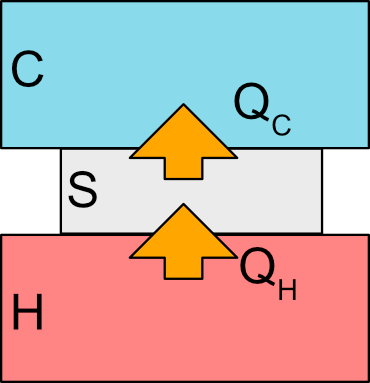
\includegraphics[width=6cm]{system} \caption{System (S) model}
\label{Fig2} 
\end{figure}

Treating the heater and the cooler as the environment, we can think of our system $S$ as an open system.
Further on we'll analyze the system $S$ from the perspective of internal $(i)$ entropy production
and external $(e)$ entropy flux, flowing \emph{to} the system $S$. 
Of course the change in entropy will be the sum of those two contributions:
\begin{equation}
dS_S=dS_i+dS_e.
\label{entrosum}
\end{equation}

In the current analysis let's consider a situation in which the same amount of heat flows in as flows out, that is $dQ_C=-dQ_H$. Using this relation we get the following term for the change of entropy:
\begin{equation}
dS_e=\frac{dQ_H}{T_H}+\frac{dQ_C}{T_C}=dQ_H\left(\frac{1}{T_H}-\frac{1}{T_C}\right)
=dQ_H\left(\frac{T_C-T_H}{T_HT_C}\right)<0.
\label{dSe1}
\end{equation}
From which it follows, that the heat flow takes the entropy out of our system.
For the purpose of further discussion we introduce the concept of rate of entropy change connected with the heat flow:
\begin{equation}
j_e \equiv  \frac{dS_e}{dt}. 
\end{equation}
In the considered scenerio, the $j_e$ is held constant (steady-state) and we suspect a continuous fall in system's entropy

Yet, moving away from the equilibrium state we suspect, that the a major role will be played by $dS_i$ moving the system back to equilibrium state. Similarly, as before we define the rate of internal entropy production:

\begin{equation}
j_i \equiv \frac{dS_i}{dt}.   
\end{equation} 

When $T_H=T_C$, i.e. the system is in equilibrium with constant entropy $S_{EQ}$ then it follows that $j_i=0$.
Therefore the rate of internal entropy production $j_i$ should be a function  of system's entropy $S_S$, i.e. $j_i = j_i(S_S)$ with the boundary condition $j_i(S_S=S_{EQ})=0$. 

Near the equilibrium state $S_S=S_{EQ}$, we can Taylor expand the function $j_i(S_S)$ to it's linear term
\begin{equation}
j_i(S_S)=j_i\left(S_{EQ}\right)+\left(S_S-S_{EQ}\right)C_1+\mathcal{O}\left(S_S^2\right),
\end{equation} 
fulfilling $j_i\left(S_{EQ}\right)=0$. 

The dimensional and stability analysis tells us that $C_1$ has the dimension of inverse time and in the case of 
$j_e=0$ should simply be equal to $S_{EQ}$, therefore:

Using the equation (\ref{entrosum}) we get
\begin{equation}
\frac{dS_S}{dt}=j_i\left(S_S\right)=\left(S_S-S_{EQ}\right)C_1, 
\label{stab}
\end{equation} 
Now we set $C_1 = -\frac{1}{\tau}$, where $\tau$ is a positive defined relaxation constant.

The solution of the equation (\ref{stab}) is then
\begin{equation}
S_S(t) =S_{EQ}+(S_0-S_{EQ})e^{-t/\tau}, 
\end{equation}
where the initial condition was set $S_S(0)=S_0$.


Now we include the term $j_e$ into our considerations.
In this case the equation (\ref{entrosum}) results in the following 
\begin{equation}
\frac{dS_S}{dt}=j_e + j_i\left(S_S\right)=j_e +\frac{S_{EQ}-S_S}{\tau}.
\label{dSSdt}
\end{equation} 

 
Given a boundary condition $S_S(0) =S_{EQ}$ it has a solution
\begin{equation}
S_S(t)=S_{EQ}+j_e\tau \left(1-e^{-t/\tau }\right),
\end{equation} 
where $j_e$ is a negative constant (graph of this function is presented on \ref{Fig4}). 
In the limit $t\rightarrow \infty$ the entropy of the system falls to the minimal value
\begin{equation}
S_{min}=S(t\rightarrow \infty) =S_{EQ}+j_e \tau < S_{EQ}.
\end{equation}

\begin{figure}[ht!]
\centering 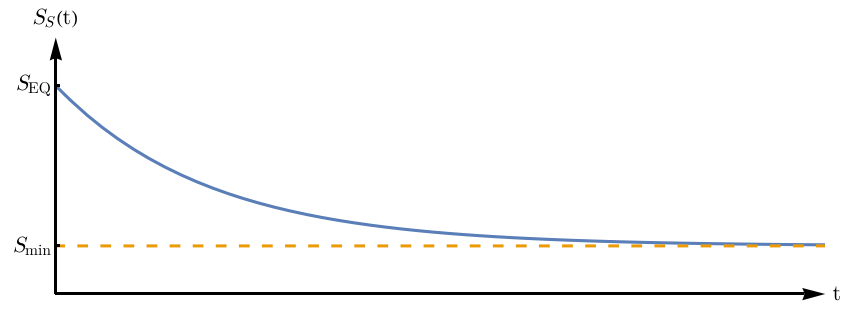
\includegraphics[width=12cm]{wykres3} 
\caption{Inducing lower entropy with heat flow.}
\label{Fig4} 
\end{figure}

This is of course consistent with the second law of thermodynamics as we're describing an open system.
It's easy to notice that the total entropy change is equal to $dS=dS_i \geq 0$ (for simplicity it was assumed that the heater and cooler don't act as producers of entropy).


\subsection{MaxEnt}

The essence of MaxEnt method can be summarized in the formula for maximization of relative entropy (negative Kullback-Leibler divergence)

\begin{displaymath}
  H(p\lor q) = -\sum_i \ln p_i \frac{p_i}{q_i}
\end{displaymath}
with respect to $p_i$ (new aposteriori distribution). $H(p||q)$ can be interpreted as the information gained by using $p_i$ instead of $q_i$.


\subsection{Near equilibrium results and concepts}

\subsubsection{Theory of Fluctuations}

Let us consider an adiabatically insulated system and a number of variables $x^i (i=1,...,n)$ which in the equilibrium state assume values $ x_0^i $, we can account for small variations ($\alpha^i$) by setting

\begin{displaymath}
  x^i = x_0^i + \alpha^i.
\end{displaymath}

The entropy in a state differing from the equilibrium state will be $S=S_0+\Delta S$, where $\Delta S$ is of the form

\begin{displaymath}
  \Delta S = - \frac{1}{2} \sum_{i,k} S_{ik} \alpha^i \alpha^k
\end{displaymath}
where $ S_{ik} $ is a positive definite form. The probability distribution for the $\alpha^i$ is given by

\begin{displaymath}
  W(\alpha^1,...,\alpha^n)d\alpha^1 ... d\alpha^1= \frac{e^{k_B \Delta S} d\alpha^1...d\alpha^n}{\int ... \int e^{k_B \Delta S} d\alpha^1...d\alpha^n}
\end{displaymath}

where $k_B$ is Boltzmann's constant.

Define

\begin{equation}
\gamma_i =\sum_k S_{ik} \alpha^k; \label{gammai}	
\end{equation}
  

then it is easily shown that

\begin{equation}
\langle \gamma_i \alpha^l \rangle = k_B \delta_i^l	
\end{equation}

Assuming ergodicity, this average may be interpreted either as an average over a microcanonical ensemble of systems, or as a time average for one single system.
By solving eq. \ref{gammai} for $\alpha^i $ we get

\begin{equation}
  \alpha^i=\sum_l S^{il}\gamma_l,
\end{equation}
and thus we find

\begin{equation}
	\langle \alpha^i \alpha^j \rangle = k_B S^{ij}   
\end{equation}

Let's suppose that $\alpha^i$ are even functions of the particle velocities with respect to time reversal.
The fact that its average future behaviour is identical to it's average past behaviour can be expressed by the equation:

\begin{equation}
  \langle \alpha^k (t+\tau)_{\alpha^{i \neq k}} \rangle =   \langle \alpha^k(t-\tau)_{\alpha^{i \neq k}} \rangle
\end{equation}

where the suffixes denote the values that remain fixed. Multiplying by $\alpha^l(t)$ and taking the average, we find

\begin{equation}
  \langle \alpha^l(t) \alpha^k (t+\tau) \rangle = \langle \alpha^l(t) \alpha^k(t-\tau) \rangle
\end{equation}

In a similar manner, for odd functions of velocities we get

\begin{equation}
  \langle \beta^l(t) \beta^k (t+\tau) \rangle = \langle - \beta^l(t) \beta^k(t-\tau) \rangle
\end{equation}

and also (by mixing odd and even functions) we get

\begin{equation}
  \langle \alpha^l(t) \beta^k (t+\tau) \rangle = \langle - \alpha^l(t) \beta^k(t-\tau) \rangle
\end{equation}

Those relations hold for all phenomena with the exception of coriolis and magnetic forces, but if we'd inverse those as well then the relations continue to hold.

By rewritting the macroscopic equations, which are of the form

\begin{equation}
  \dot{\alpha^i}= \sum_k L_k^i \alpha_k
\end{equation}

into the form

\begin{equation}
  \dot{\alpha^i}= \sum_k p^{ik} \gamma_k
\end{equation}

We assume that the same equations also describe the average behaviour of fluctuations in the following sense: there exists a time interval $\tau_1$ suchthat for $\tau > \tau_1$, but $\tau \ll T$, where $T$ is the time in which, according to our equations, a disturbance of equilibrium is appreciably reduced; then

\begin{equation}
    \langle \alpha^l(t+\tau)- \alpha^l (t) \rangle = \tau \sum_k p^{ik} \gamma_k(t).
\end{equation}
		

\paragraph{Relation to detailed balance}

The principle of detailed balance is formulated for kinetic systems which are decomposed into elementary processes
\subsubsection{Reciprocal relations}

\subsubsection{Green-Kubo relations}


\subsection{Prigogine's MinEP}
Prigogine himself noted \cite{Prigogine:1979ul}:
"It came as a great surprise when it was shown that in systems far from equilibrium the thermodynamic behavior could be quite different-in fact, even directly opposite that predicted by the theorem of minimum entropy production."

Dewar and Maritan \cite{Dewar:2014ek} showed using Jaynes's maximum entropy method that a state of minimum dissipation (MinEP) is selected for a system without dynamic instability, whereas that of maximum dissipation (MaxEP) is selected for a system with dynamic instability.

\newpage

\section{Concepts of non-equilibrium thermodynamics}
The term "irreversible process" is synonymous with a specific direction of time.
To our best knowledge the specific direction of time we experience is an emergent phenomena.
Isolated thermodynamic systems evolve in the direction of more probable states i.e. positive dissipation (larger entropy).
When they finally reach that state the direction of time ceases to exist for the whole system. 
Therefore in the description of irreversible processes the history of the system evolution becomes relevant.


\subsection{Local equilibrium}
The thermodynamical variables are often defined subject to the kinematical requirement of local thermodynamic equilibrium. This means that collisions between molecules are so frequent that chemical and radiative processes do not disrupt the local Maxwell-Boltzmann distribution of molecular velocities. This principle is valid for hydrodynamic flows and chemical reactions and it's formulation goes back to Clark Maxwell [Citation?].
It's usage can be usually justified by assuming analyticity of thermodynamic state functions arbitrarily close to equilibrium - then, local equilibrium is obtained from first order expansion of thermodynamic properties in the irreversible fluxes ${X_i}$ \cite{Evans:2002gg}.

\subsubsection{Definition of temperature}
When the temperature differences are "smooth" enough, i.e., locally there is a reasonable definition of temperature (local equilibrium), then the temperature gradient determines the heat flux. In the opposite case, it is molecular kinetics who determines the energy transfer. The latter happens much faster and local equilibrium gets established quickly.

On the other hand, far from equilibrium there might be a problem defining temperature and also Clausius entropy which depends on it. One of the solutions provided by Evans at al in  is to define temperature of non equilibrium state by the temperature of the target equilibrium state to which the system would otherwise relax.

\subsection{Entropy production}

In near equilibrium regime, where local thermodynamic equilibrium is expected to be valid, the theory predicts that there will be a 'spontaneous production of entropy' in non-equilibrium systems.
This spontaneous production of entropy is given by the entropy production per unit volume $\sigma$ by the following expression \cite{DeGroot:1984ue}
\begin{displaymath}
  \int d\bm{r} \sigma(\bm{r},t)=\int d\bm{r}(\sum_i J_i(\bm{r},t)X_i(\bm{r},t))>0,
\end{displaymath}
where $J_i(\bm{r},t)$ are the Navier-Stokes hydrodynamic fluxes (e.g. the stress tensor, heat flux vector,...) at position $\bm{r}$ and time $t$ and $X_i$ is the thermodynamic force which is conjugate to $J_i(\bm{r},t)$ (e.g. strain rate tensor divided by temperature or the gradient of the reciprocal of temperature,... respectively).

Limitations:

\subsection{Steady states}
The most basic of non-equilibrium conditions, the steady state is already difficult to describe as may of the basic state functions (including temperature and entropy), are undefined for far from equilibrium states and the distribution function of a steady state is fractal and non-analytic. 


\subsection{Dissipation}

If external fields are applied to the system of particles and the external field does work on the system and if that work can be turned completely into heat that can diffuse out of the system, the external field is termed a dissipative field. If the work can be completely stored in the system in the form of potential energy, the external field is termed non-dissipative.

A simple example of a system that turns from non-dissipative into a dissipative system is sodium chloride. In solid state it's an insulator (internal energy increases through polarization), but when heated to around 1100K, melts and becomes a conductor.

\subsection{Condition of adiabatic incompressibility of phase space}

We say that a system fulfills the \textit{adiabatic incompressibility of phase space} or $AI\Gamma$ if in the absence of the thermostatting terms the equations of motion preserve the phase space volume, that is
\begin{equation}
  \Lambda \equiv (\partial / \partial\bm{\Gamma}) \cdot \dot{\bm{\Gamma}}=0
\end{equation}

\section{General properties of non-equilibrium systems}

\subsection{Driven systems}

A subcategory of non-equilibrium systems are those that we call \textit{driven}.
Those systems, composed of interacting particles and possibly thermostatted, are subject to an external dissipative field $F_e$.


\section{Non-equilibrium results}
There exist only a handful of relations correct arbitrarily far from equilibrium, these include:
\begin{itemize}
  \item Jarzynski non-equilibrium work relation
  \item Kawasaki relation
  \item Evans-Searles transient fluctuation theorem
\end{itemize}
Those relations have several commonalities:
\begin{itemize}
  \item the system starts in thermal equilibrium
  \item it is driven from that equilibrium by an external perturbation
  \item the energy of the system always remains finite
  \item the dynamics are markovian 
  \item if the system is unperturbed then the dynamics preserve the equilibrium ensemble
\end{itemize}
It's clear from that a system with these properties is microscopically reversible.

All those relations can be considered a special cases of a single theorem


\subsection{Dissipation function}

Dissipation function was first properly (not implicitly) defined in 2000 by Searles and Evans 

The instantaneous dissipation function:

\begin{equation}
  \Omega(\Gamma)=-\frac{1}{f(\bm{\Gamma};0)}\dot{\bm{\Gamma}}(\bm{\Gamma})\frac{\partial{f(\bm{\Gamma};0)}}{\partial{\bm{\Gamma}}}-\Lambda(\bm{\Gamma})
\end{equation}


\begin{displaymath}
  \Omega_t(\Gamma(t))=\frac{d \Omega_t(\Gamma(0))}{dt}
\end{displaymath}


\begin{displaymath}
  \Omega_t(\Gamma(0))=ln{\frac{P(\Gamma(0),0)}{P(\Gamma^*(t),0)}}
\end{displaymath}

The dissipation function is similar to the entropy production, and although it's not a state function it provides description of non-equilibrium systems through various fluctuation theorems.

\subsubsection{Derivation}


\begin{equation}
\begin{aligned}
  f(S^t\bm{\Gamma};t) &= exp[-\int_0^t ds\ \Lambda(S^s\bm{\Gamma})]f(\bm{\Gamma};0)\\
  &=exp[-\int_0^t ds\ \Lambda(S^s\bm{\Gamma})]f(S^t \bm{\Gamma};0) exp[\int_0^t ds\ \Omega(S^s \bm{\Gamma}) + \int_0^t ds\ \Lambda(S^s\bm{\Gamma})]\\
  &=f(S^t \bm{\Gamma};0) exp[\int_0^t ds\ \bm{\Omega}(S^s \bm{\Gamma})]
\end{aligned}
\end{equation}


\subsection{Fluctuation Theorem}
The Fluctuation Theorem is best regarded as a set of closely related theorems.
One of the reason for this situation is because we'd expect different fluctuations for different statistical mechanical ensembles.
Second reason, because of which we've got this diversity is that some of this theorems refer to non-equilibrium steady state fluctuations (e.g.), while others refer to transient fluctuations.
For the needs of this we will further refer to Steady State Fluctuation Theorems (SSFT) valid in the long averaging times and Transient Fluctuation Theorems (TFT) which are exact for arbitrary averaging times.

\subsubsection{Evans-Searles Fluctuation Theorem}
Evans-Searles Fluctuation Theorem results in a generalisation of the Second Law of Thermodynamics so that it applies to small systems, including those that evolve far from equilibrium.
It describes how a finite sized system's irreversibility develops in time from a completely time-reversible system at short observation times, to an irreversible one at long times or when the system's size increases. 
...

We have now completed our derivation of the Transient Fluctuation Theorem
\begin{displaymath}
  \frac{p(\Omega_t=A)}{p(\Omega_t=-A)}=exp(A t)
\end{displaymath}


If we're interested in steady state then we'll allow the system for some relaxation time $\tau_r$

\begin{displaymath}
  lim_{\frac{t}{\tau_R}\rightarrow \infty} \frac{1}{t} ln{\frac{p(\Omega_{t,ss}=A)}{p(\Omega_{t,ss}=-A)}} =A
\end{displaymath}


The fluctuation theorem relates the probabilities of observing time averaged values of a generalized entropy production (dissipation function), for a time period t.

\begin{displaymath}
  \Omega(\Gamma) \equiv \ln \left(\frac{f(\Gamma ,0)}{f(\Gamma  t,0)}\right)+\underset{0}{\overset{t}{\int }}\frac{\left(\dot{Q} s\right) ds}{k_B T_{\text{res}}}
\end{displaymath}

\subsubsection{Crooks Fluctuation Theorem}

Crooks Fluctuation Theorem, provides a method of predicting equilibrium free energy difference from ex- perimental information taken from nonequilibrium paths that connect two equi- librium states. This FT can be used to derive the well known Jarzynski Equality, which expresses the free energy difference between two equilibrium states in terms of an average over irreversible paths.

\subsubsection{As a measure of irreversibility}
If we denote T as irreversibility then I can be interpreted as a measure of T-symmetry breaking.
\begin{displaymath}
  I =\int p(x) \ln{\frac{p( x)}{p(T x)}}
\end{displaymath}


\subsection{Dissipation Theorem}
The Dissipation Theorem says that the nonlinear response of an arbitrary phase variable can be calculated from the time integral of the non-equilibrium transient time correlation function of the phase variable with the dissipation function


\begin{equation}
\langle B(t)\rangle =\langle B(0) \rangle +\int_0^t ds \langle B(s) \Omega(0) \rangle \label{disstheo}
\end{equation}

A simple consequence of this theorem can be read of immediately that is, for equilibrium (lack of dissipation) the ensemble averages stay constant.

In systems in which the external field drives the system out of equilibrium in a linear manner (weak field), Eq. \ref{disstheo} reduces to Green-Kubo linear response relation.

\subsubsection{Derivation}

\subsubsection{$\Omega T$ Mixing}

We say that a system possesses the property of $\Omega T$ mixing if the integral
\begin{equation}
  \int_0^t ds \langle B(s) \Omega(0) \rangle
\end{equation}
is bounded from above. This requirement let's us predict that the system will relax either to a non-equilibrium steady state or toward an equilibrium.

This property is more restrictive than $T$ mixing known from ergodic theory, therefore if a system is $\Omega T$ mixing it's also $T$ mixing, but not necessarily the opposite.

\subsection{Relaxation Theorem}
The Relaxation Theorem says that if an arbitrary initial ensemble of ergodic Hamiltonian systems is in contact with a heat bath and there is a decay of temporal correlations, then the system will at long times, relax to the Maxwell-Boltzmann distribution. Further, this distribution has zero dissipation everywhere in phase space. For such systems no other distribution has zero dissipation everywhere.
\begin{displaymath}
  \lim_{t\to \infty } \Omega (\Gamma ;f(\Gamma ,t))=0, \forall \Gamma
\end{displaymath}

A system can relax to equilibrium in two ways: conformally and non-conformally.
Each of the above results is exact arbitrarily far from equilibrium and independent of system size.

\subsection{Gibbs Entropy}

\subsubsection{Constancy for Hamiltonian systems}

\subsubsection{Divergence}

\section{Models of time-reversible thermostat}

The first time-reversible, deterministic thermostats and ergostats were invented in the early 1980s by Hoover, Ladd and Moran . Prior to this development there was no satisfactory mathematical way of modelling thermostatted non-equilibrium steady states. \cite{Hoover:1982dp}

\subsection{Nose-Hoover}

By including a term $-S_i \alpha \bm{p}_i $ to the EOM we get a deterministic, time-reversible Nose-Hoover thermostat, which can be used to add or remove heat from the particles in the reservoir region through introduction of an extra degree of freedom described by $\alpha$

\section{Search for a unifying principle}

The search for variational or extremization principles in physics has a long history of success. In classical mechanics, one finds the Lagrangian and Hamiltonian formalisms with the principle of least action. In thermodynamics and statistical physics of equilibrium state the principle of maximum entropy reigns. 

In 1912, Ehrenfest was the first who asked whether such a principle for a yet unknown function could exist for non-equilibrium steady states. 

This approach has also gained a lot of criticism.
On the other hand, according to Kondepudi (2008),[7] and to Grandy (2008),[8] there is no general rule that provides an extremum principle that governs the evolution of a far-from-equilibrium system to a steady state. 
Silhavy (1997)[11] offers the opinion that "... the extremum principles of thermodynamics ... do not have any counterpart for [non-equilibrium] steady states (despite many claims in the literature)." It follows that any general extremal principle for a non-equilibrium problem will need to refer in some detail to the constraints that are specific for the structure of the system considered in the problem.

There seems to be a theoretical relationship between maximum irreversibility and dynamic stability [Beyond the Second Law] a link suggested here by the fact that MaxEnt/MaxEP predicts the same dissipation functional as Malkus's instability criterion in shear turbulence

\subsection{Rayleigh's insight}
Studying jets of water from a nozzle, Rayleigh (1878,[27] 1896/1926[28]) noted that when a jet is in a state of conditionally stable dynamical structure, the mode of fluctuation most likely to grow to its full extent and lead to another state of conditionally stable dynamical structure is the one with the fastest growth rate. In other words, a jet can settle into a conditionally stable state, but it is likely to suffer fluctuation so as to pass to another, less unstable, conditionally stable state. He used like reasoning in a study of Benard convection.[39] These physically lucid considerations of Rayleigh seem to contain the heart of the distinction between the principles of minimum and maximum rates of dissipation of energy and entropy production, which have been developed in the course of physical investigations by later authors.

\subsection{Current state of affairs}

- near equilibrium least dissipation
- near-equilibrium minEP
- near-equilibrium maxEP
- far from equilibrium non-variational maxEP
- far from equilibrium variational maxEP and optimization EP

far from equilibrium usually means far from global equilibrium near local equilibrium.

\subsection{MEP}
\subsubsection{Relation between fluctuation theorem and MEP}
\subsubsection{Results for atmospheres?}
\section{Physics of adaptation and self-replication}

\section{Statistical measures of complexity}
\subsection{Kolmogorov complexity}

\subsection{Growth of complexity}


[In quantum computation, the notion of complexity refers to the minimum number of gates needed to prepare a certain state from a reference state. This pragmatic notion has now been related to something more exotic: black hole horizons. More precisely, it has been conjectured that the growth of the volume of a black hole interior is dual to the growth in computational complexity. Adam Brown and colleagues revisited this conjecture and restated it, this time relating complexity to the action of a particular type of spacetime region called a Wheeler DeWitt patch. In other words, the computational complexity of a boundary relates to the geometry of a bulk region.
There are reasons to believe that the original conjecture, and hence the new one, is likely to be correct. Interestingly, the new conjecture may have deeper implications connecting quantum information and quantum gravity. And it also suggests that black holes could reach the physical limits of computation determined by the fundamental constants. In this sense, black holes are the fastest computers in the known universe.]

\bibliographystyle{ieeetr}
\bibliography{Refs}


\end{document}